\documentclass[11pt]{article}
\usepackage{palatino}
\usepackage{latexsym}
\usepackage{verbatim}
\usepackage{alltt}
\usepackage{amsmath,proof,amsthm,amssymb,enumerate,mathabx}
\usepackage[margin=1.0in]{geometry}
\usepackage{math-cmds}
\usepackage{listings}
\usepackage{tkz-graph}


\newcommand{\definition}[2]
  {\bigskip \noindent
   \textbf{Definition (#1).}  #2
   \bigskip
  }
  
\newcommand{\exercise}[1]
  {\bigskip \noindent
   {\bf Exercise #1}.}

\newcommand{\printanswer}[1]
  {}   % use {#1} to print answers, {} to omit them
   
\newcommand{\answer}[2]
  {\bigskip \printanswer{\noindent
   {\bf Sample Answer #1}. #2 \bigskip}}
   
\newcommand{\parg}[1] % program argument
  {\ldbrack #1 \rdbrack}

\def\tablespace{\vspace{2ex}}



\def\prop{\textsf{\,\,prop}}
\def\thm{\textsf{\,\,thm}}
\def\implies{\Rightarrow}

\newcommand{\join}{\sqcup}
\newcommand{\meet}{\sqcap}
\newcommand{\alap}{\sqsubseteq}
\newcommand{\todo}[1]{}


\title{Lecture Notes:
		Pointer Analysis}
\author{15-819O: Program Analysis \emph{(Spring 2016)} \\
        Claire Le Goues \\
		{\tt clegoues@cs.cmu.edu}}
\date{}

\begin{document}
\begin{sloppypar}
\newtheorem{theorem}{Theorem}
\newtheorem{lemma}[theorem]{Lemma}

\maketitle

\section{Motivation for Pointer Analysis}

In the spirit of extending our understanding of analysis to more realistic languages, consider programs with pointers, or variables whose value refers to another value stored elsewhere in memory by storing the address of that stored value.  Pointers are very common in imperative and object-oriented programs, and ignoring them can dramatically impact the precision of other analyses that we have discussed.  Consider constant-propagation analysis of the following program:

\[
\begin{array}{ll}
1: & z := 1\\
2: & p := \&z\\
3: & *p := 2\\
4: & \mbox{print}~ z\\
\end{array}
\]

\noindent To analyze this program correctly we must be aware that at instruction 3 $p$ points to $z$.  If this information is available we can use it in a flow function as follows:

\[
\begin{array}{lll}

f_{CP}\parg{*p := y}(\sigma) & = [z \mapsto \sigma(y)]\sigma & \mbox{where}~ \textit{must-point-to}(p,z)\\[1ex]

\end{array}
\]

When we know exactly what a variable $x$ points to, we have \textit{must-point-to} information, and we can perform a \textit{strong update} of the target variable $z$, because we know with confidence that assigning to $*p$ assigns to $z$.  A technicality in the rule is quantifying over all $z$ such that $p$ must point to $z$.  How is this possible?  It is not possible in C or Java; however, in a language with pass-by-reference, for example C++, it is possible that two names for the same location are in scope.

Of course, it is also possible to be uncertain to which of several distinct locations $p$ points:

\[
\begin{array}{ll}
1: & z := 1\\
2: & \mathbf{if}~ (\textit{cond})~ p := \&y ~\mathbf{else}~ p := \&z\\
3: & *p := 2\\
4: & \mathbf{print}~ z\\
\end{array}
\]

Now constant propagation analysis must conservatively assume that $z$ could hold either 1 or 2.  We can represent this with a flow function that uses may-point-to information:

\[
\begin{array}{lll}

f_{CP}\parg{*p := y}(\sigma) & = [z \mapsto \sigma(z) \join \sigma(y)]\sigma & \mbox{where}~ \textit{may-point-to}(p,z)\\[1ex]

\end{array}
\]

\section{Andersen's Points-To Analysis}

Two common kinds of pointer analysis are alias analysis and points-to analysis.  Alias analysis computes sets $S$ holding pairs of variables $(p,q)$, where $p$ and $q$ may (or must) point to the same location.  Points-to analysis, as described above, computes a relation $\textit{points-to}(p,x)$, where $p$ may (or must) point to the location of the variable $x$.  We will focus primarily on points-to analysis, beginning with a simple but useful approach originally proposed by Andersen (PhD thesis: ``Program Analysis and Specialization for the C Programming Language").

Our initial setting will be C programs.  We are interested in analyzing instructions that are relevant to pointers in the program.  Ignoring for the moment memory allocation and arrays, we can decompose all pointer operations into four  types: taking the address of a variable, copying a pointer from one variable to another, assigning through a pointer, and dereferencing a pointer:

\[
\begin{array}{lll}
I & \bnfdef & ... \\
  & \bnfalt & p := \&x \\
  & \bnfalt & p := q \\
  & \bnfalt & *p := q \\
  & \bnfalt & p := *q \\
\end{array}
\]

Andersen's points-to analysis is a context-insensitive interprocedural analysis.  It is also a \textit{flow-insensitive analysis}, that is an analysis that does not consider program statement order.  Context- and flow-insensitivity are used to improve the performance of the analysis, as precise pointer analysis can be notoriously expensive in practice.

We will formulate Andersen's analysis by generating set constraints which can later be processed by a set constraint solver using a number of technologies.  Constraint generation for each statement works as given in the following set of rules.  Because the analysis is flow-insensitive, we do not care what order the instructions in the program come in; we simply generate a set of constraints and solve them.

\[
\begin{array}{c}
\infer[\textit{address-of}]
	{\parg{p := \&x} \hookrightarrow l_x \in p}
	{}\\[3ex]
	
\infer[\textit{copy}]
	{\parg{p := q} \hookrightarrow p \supseteq q}
	{}\\[3ex]
	
\infer[\textit{assign}]
	{\parg{*p := q} \hookrightarrow *p \supseteq q}
	{}\\[3ex]
	
\infer[\textit{dereference}]
	{\parg{p := *q} \hookrightarrow p \supseteq *q}
	{}\\[3ex]
	
\end{array}
\]

The constraints generated are all set constraints.  The first rule states that a constant location $l_x$, representation the address of $x$, is in the set of location pointed to by $p$.  The second rule states that the set of locations pointed to by $p$ must be a superset of those pointed to by $q$.  The last two rules state the same, but take into account that one or the other pointer is dereferenced.

A number of specialized set constraint solvers exist and constraints in the form above can be translated into the input for these.  The dereference operation (the $*$ in $*p \supseteq q$) is not standard in set constraints, but it can be encoded---see F\"ahndrich's Ph.D. thesis for an example of how to encode Andersen's points-to analysis for the BANE constraint solving engine.  We will treat constraint-solving abstractly using the following constraint propagation rules:

% COME UP WITH THESE BY EXAMPLE IN CLASS

\[
\begin{array}{c}
\infer[\textit{copy}]
	{l_x \in p}
	{p \supseteq q & l_x \in q}\\[3ex]
		
\infer[\textit{assign}]
	{l_x \in r}
	{*p \supseteq q & l_r \in p & l_x \in q}\\[3ex]
	
\infer[\textit{dereference}]
	{l_x \in p}
	{p \supseteq *q & l_r \in q & l_x \in r}\\[3ex]
	
\end{array}
\]

We can now apply Andersen's points-to analysis to the program above.  Note that in this example if Andersen's algorithm says that the set $p$ points to only one location $l_z$, we have must-point-to information, whereas if the set $p$ contains more than one location, we have only may-point-to information.

We can also apply Andersen's analysis to programs with dynamic memory allocation, such as:

\[
\begin{array}{ll}
1: & q := \textit{malloc}_1()\\
2: & p := \textit{malloc}_2()\\
3: & p := q\\
4: & r := \&p\\
5: & s := \textit{malloc}_3()\\
6: & *r := s\\
7: & t := \&s\\
8: & u := *t\\
\end{array}
\]

In this example, the analysis is run the same way, but we treat the memory cell allocated at each \textit{malloc} or \textit{new} statement as an abstract location labeled by the location $n$ of the allocation point.  We can use the rules:

\[
\begin{array}{c}
\infer[\textit{malloc}]
	{\parg{p := \textit{malloc}_n()} \hookrightarrow l_n \in p}
	{}\\[3ex]
	
\end{array}
\]

We must be careful because a \textit{malloc} statement can be executed more than once, and each time it executes, a new memory cell is allocated.  Unless we have some other means of proving that the malloc executes only once, we must assume that if some variable $p$ only points to one abstract malloc'd location $l_n$, that is still may-alias information (i.e. $p$ points to only one of the many actual cells allocated at the given program location) and not must-alias information.

Analyzing the efficiency of Andersen's algorithm, we can see that all constraints can be generated in a linear $O(n)$ pass over the program.  The solution size is $O(n^2)$ because each of the $O(n)$ variables defined in the program could potentially point to $O(n)$ other variables.

We can derive the execution time from a theorem by David McAllester published in SAS'99.  There are $O(n)$ flow constraints generated of the form $p \supseteq q$, $*p \supseteq q$, or $p \supseteq *q$.  How many times could a constraint propagation rule fire for each flow constraint?  For a $p \supseteq q$ constraint, the rule may fire at most $O(n)$ times, because there are at most $O(n)$ premises of the proper form $l_x \in p$.  However, a constraint of the form $p \supseteq *q$ could cause $O(n^2)$ rule firings, because there are $O(n)$ premises each of the form $l_x \in p$ and $l_r \in q$.  With $O(n)$ constraints of the form $p \supseteq *q$ and $O(n^2)$ firings for each, we have $O(n^3)$ constraint firings overall.  A similar analysis applies for $*p \supseteq q$ constraints.  McAllester's theorem states that the analysis with $O(n^3)$ rule firings can be implemented in $O(n^3)$ time.  Thus we have derived that Andersen's algorithm is cubic in the size of the program, in the worst case.

\todo{add citation to McAllester}

\subsection{Field-Sensitive Analysis}

What happens when we have a pointer to a struct in C, or an object in an object-oriented language? In this case, we would like the pointer analysis to tell us what each field in the struct or object points to.
%
A simple solution is to be \textit{field-insensitive}, treating all fields in a struct as equivalent. Thus if $p$ points to a struct with two fields $f$ and $g$, and we assign:

\[
\begin{array}{ll}
1: & p.f := \&x\\
2: & p.g := \&y\\
\end{array}
\]

A field-insensitive analysis would tell us (imprecisely) that $p.f$ could point to $y$.
%
In order to be more precise, we can track the contents each field of each abstract location separately.  In the discussion below, we assume a setting in which we cannot take the address of a field; this assumption is true for Java but not for C.  We can define a new kind of constraints for fields:

\[
\begin{array}{c}
\infer[\textit{field-read}]
	{\parg{p := q.f} \hookrightarrow p \supseteq q.f}
	{}\\[3ex]
	
\infer[\textit{field-assign}]
	{\parg{p.f := q} \hookrightarrow p.f \supseteq q}
	{}\\[3ex]
	
\end{array}
\]


Now assume that objects (e.g. in Java) are represented by abstract locations $l$.  We can process field constraints with the following rules:

\[
\begin{array}{c}
\infer[\textit{field-read}]
	{l_f \in p}
	{p \supseteq q.f & l_q \in q & l_f \in l_q.f}\\[3ex]
	
\infer[\textit{field-assign}]
	{l_q \in l_p.f}
	{p.f \supseteq q & l_p \in p & l_q \in q}\\[3ex]
	
\end{array}
\]

If we run this analysis on the code above, we find that it can distinguish that $p.f$ points to $x$ and $p.g$ points to $y$.


\section{Steensgaard's Points-To Analysis}

For large programs, a cubic algorithm is too inefficient.  Steensgaard proposed an pointer analysis algorithm that operates in near-linear time, supporting essentially unlimited scalability in practice.

The first challenge in designing a near-linear time points-to analysis is to represent the results in linear space.  This is nontrivial because over the course of program execution, any given pointer $p$ could potentially point to the location of any other variable or pointer $q$.  Representing all of these pointers explicitly will inherently take $O(n^2)$ space.

The solution Steensgaard found is based on using constant space for each variable in the program.  His analysis associates each variable $p$ with an abstract location named after the variable.  Then, it tracks a single points-to relation between that abstract location $p$ and another one $q$, to which it may point.  Now, it is possible that in some real program $p$ may point to both $q$ and some other variable $r$.  In this situation, Steensgaard's algorithm \textit{unifies} the abstract locations for $q$ and $r$, creating a single abstract location representing both of them.  Now we can track the fact that $p$ may point to either variable using a single points-to relationship.

For example, consider the program below:

\[
\begin{array}{ll}
1: & p := \&x\\
2: & r := \&p\\
3: & q := \&y\\
4: & s := \&q\\
5: & r := s\\
\end{array}
\]

Andersen's points-to analysis would produce the following graph:

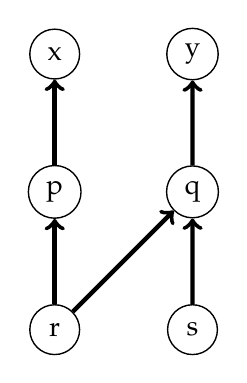
\begin{tikzpicture}[scale=1.75]
\GraphInit[vstyle=Normal]
\Vertex{x}
\Vertex[x=0,y=-1]{p}
\Vertex[x=0,y=-2]{r}
\Vertex[x=1,y= 0]{y}
\Vertex[x=1,y=-1]{q}
\Vertex[x=1,y=-2]{s}
\SetUpEdge[style={->,ultra thick}]
\Edges(r,p,x)
\Edges(s,q,y)
\Edge(r)(q)
\end{tikzpicture}

But in Steensgaard's setting, when we discover that $r$ could point both to $q$ and to $p$, we must merge $q$ and $p$ into a single node:

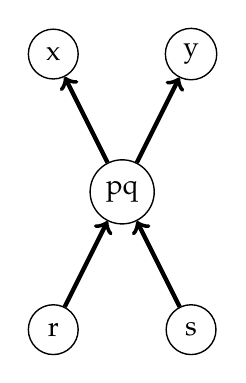
\begin{tikzpicture}[scale=1.75]
\GraphInit[vstyle=Normal]
\Vertex{x}
\Vertex[x=0.5,y=-1]{pq}
\Vertex[x=0,y=-2]{r}
\Vertex[x=1,y= 0]{y}
\Vertex[x=1,y=-2]{s}
\SetUpEdge[style={->,ultra thick}]
\Edges(r,pq,x)
\Edges(s,pq,y)
\end{tikzpicture}

Notice that we have lost precision: by merging the nodes for $p$ and $q$ our graph now implies that $s$ could point to $p$, which is not the case in the actual program.  But we are not done.  Now $pq$ has two outgoing arrows, so we must merge nodes $x$ and $y$.  The final graph produced by Steensgaard's algorithm is therefore:

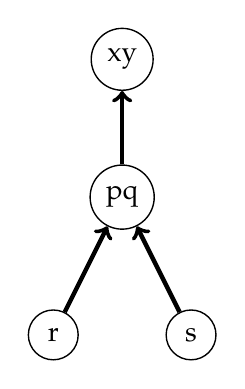
\begin{tikzpicture}[scale=1.75]
\GraphInit[vstyle=Normal]
\Vertex{xy}
\Vertex[x=0,y=-1]{pq}
\Vertex[x=-0.5,y=-2]{r}
\Vertex[x=0.5,y=-2]{s}
\SetUpEdge[style={->,ultra thick}]
\Edges(r,pq,xy)
\Edges(s,pq)
\end{tikzpicture}

To define Steensgaard's analysis more precisely, 
we will study a simplified version of that ignores function pointers.  It can be specified as follows:

\[
\begin{array}{c}
\infer[\textit{copy}]
	{\parg{p := q} \hookrightarrow \textit{join}(*p,*q)}
	{}\\[3ex]
	
\infer[\textit{address-of}]
	{\parg{p := \&x} \hookrightarrow \textit{join}(*p,x)}
	{}\\[3ex]
	
\infer[\textit{dereference}]
	{\parg{p := *q} \hookrightarrow \textit{join}(*p,*{*}q)}
	{}\\[3ex]
	
\infer[\textit{assign}]
	{\parg{*p := q} \hookrightarrow \textit{join}(*{*}p,*q)}
	{}\\[3ex]
	
\end{array}
\]

With each abstract location $p$, we associate the abstract location that $p$ points to, denoted $*p$.  Abstract locations are implemented as a union-find\footnote{See any algorithms textbook} data structure so that we can merge two abstract locations efficiently.  In the rules above, we implicitly invoke \textit{find} on an abstract location before calling \textit{join} on it, or before looking up the location it points to.

The \textit{join} operation essentially implements a union operation on the abstract locations.  However, since we are tracking what each abstract location points to, we must update this information also.  The algorithm to do so is as follows:


\begin{lstlisting}%[mathescape]

join(e1, e2)
    if (e1 == e2)
        return
    e1next = *e1
    e2next = *e2
    unify(e1, e2)
    join(e1next, e2next)

\end{lstlisting}


Once again, we implicitly invoke \textit{find} on an abstract location before comparing it for equality, looking up the abstract location it points to, or calling \textit{join} recursively.

As an optimization, Steensgaard does not perform the join if the right hand side is not a pointer.  For example, if we have an assignment $\parg{p := q}$ and $q$ has not been assigned any pointer value so far in the analysis, we ignore the assignment.  If later we find that $q$ may hold a pointer, we must revisit the assignment to get a sound result.

Steensgaard illustrated his algorithm using the following program:

\[
\begin{array}{ll}
1: & a := \&x\\
2: & b := \&y\\
3: & \mbox{if}~ p ~\mbox{then}\\
4: & ~~~~ y := \&z\\
5: & \mbox{else}\\
6: & ~~~~ y := \&x\\
7: & c := \&y\\
\end{array}
\]

His analysis produces the following graph for this program:

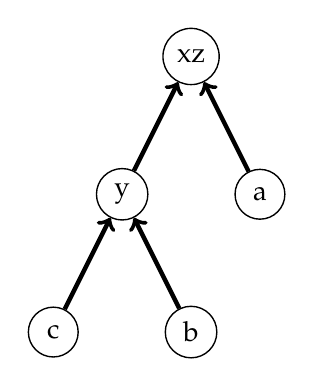
\begin{tikzpicture}[scale=1.75]
\GraphInit[vstyle=Normal]
\Vertex{c}
\Vertex[x=1,y=0]{b}
\Vertex[x=0.5,y=1]{y}
\Vertex[x=1.5,y=1]{a}
\Vertex[x=1,y=2]{xz}
\SetUpEdge[style={->,ultra thick}]
\Edges(a,xz)
\Edges(y,xz)
\Edges(b,y)
\Edges(c,y)
\end{tikzpicture}


%Rayside demonstrates the difference in precision between Andersen's and Steensgaard's analyses using the following program:

%\[
%\begin{array}{ll}
%1: & p := \textit{malloc}_1()\\
%2: & q := \textit{malloc}_2()\\
%3: & fp:= \&p\\
%4: & fp:= \&q\\
%5: & ... := *fp\\
%\end{array}
%\]


Rayside illustrates a situation in which Andersen must do more work than Steensgaard:

\todo{Cite Rayside notes}

\[
\begin{array}{ll}
1: & q := \&x\\
2: & q := \&y\\
3: & p := q\\
4: & q := \&z\\
\end{array}
\]

After processing the first three statements, Steensgaard's algorithm will have unified variables $x$ and $y$, with $p$ and $q$ both pointing to the unified node.  In contrast, Andersen's algorithm will have both $p$ and $q$ pointing to both $x$ and $y$.  When the fourth statement is processed, Steensgaard's algorithm does only a constant amount of work, merging $z$ in with the already-merged $xy$ node.  On the other hand, Andersen's algorithm must not just create a points-to relation from $q$ to $z$, but must also propagate that relationship to $p$.  It is this additional propagation step that results in the significant performance difference between these algorithms.

Analyzing Steensgaard's pointer analysis for efficiency, we observe that each of $n$ statements in the program is processed once.  The processing is linear, except for \textit{find} operations on the union-find data structure (which may take amortized time $O(\alpha(n))$ each) and the \textit{join} operations.  We note that in the \textit{join} algorithm, the short-circuit test will fail at most $O(n)$ times---at most once for each variable in the program.  Each time the short-circuit fails, two abstract locations are unified, at cost $O(\alpha(n))$.  The unification assures the short-circuit will not fail again for one of these two variables.  Because we have at most $O(n)$ operations and the amortized cost of each operation is at most $O(\alpha(n))$, the overall running time of the algorithm is near linear: $O(n * \alpha(n))$.  Space consumption is linear, as no space is used beyond that used to represent abstract locations for all the variables in the program text.

Based on this asymptotic efficiency, Steensgaard's algorithm was run on a 1 million line program (Microsoft Word) in 1996; this was an order of magnitude greater scalability than other pointer analyses known at the time.

Steensgaard's pointer analysis is field-insensitive; making it field-sensitive would mean that it is no longer linear.


\section{Adding Context Sensitivity to Andersen's Algorithm}

We can define a version of Andersen's points-to algorithm that is context-sensitive.  In the following approach, we analyze each function separately for each calling point.  The analysis keeps track of the current context, the calling point $n$ of the current procedure.  In the constraints, we track separate values for each variable $x_n$ according to the calling context $n$ of the procedure defining it, and we track separate values for each memory location $l^k_n$ according to the calling context $n$ active when that location was allocated at new instruction $k$.  The rules are as follows:

\[
\begin{array}{c}
\infer[\textit{new}]
	{l^k_n \in p_n}
	{n \vdash p := \mathbf{new}_k~A}\\[3ex]

\infer[\textit{copy}]
	{l_n \in p_n}
	{n \vdash p := q & l_n \in q_n}\\[3ex]
		
\infer[\textit{field-read}]
	{l_y \in l_x.f}
	{n \vdash x.f := y & l_x \in x_n & l_y \in y_n}\\[3ex]
	
\infer[\textit{field-assign}]
	{l_z \in x_n}
	{n \vdash x := y.f & l_y \in y_n & l_z \in l_y.f}\\[3ex]
	
\infer[\textit{call}]
	{l_y \in z_k ~~~~ k \vdash e}
	{n \vdash f_k(y) & l_y \in y_n & \parg{f(z) = e} \in \mathit{Program}}\\[3ex]
	
\end{array}
\]

To illustrate this analysis, imagine we have the following code:

\begin{lstlisting}
interface A { void g(); }
class B implements A { void g() { ... } }
class C implements A { void g() { ... } }
class D {
    A f(A a1) { return a1; }
}

// in main()
D d1 = new D();
if (...) {
    A x = d1.f(new B());
	x.g() // which g is called?
else
    A y = d1.f(new C());
	y.g() // which g is called?
\end{lstlisting}

The analysis produces the following aliasing graph:

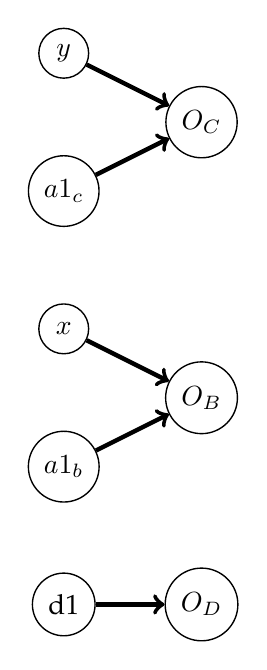
\begin{tikzpicture}[scale=1.75]
\GraphInit[vstyle=Normal]
\Vertex{d1}
\Vertex[x=1,y=0]{$O_D$}
\Vertex[x=0,y=1]{$a1_b$}
\Vertex[x=1,y=1.5]{$O_B$}
\Vertex[x=0,y=2]{$x$}
\Vertex[x=0,y=3]{$a1_c$}
\Vertex[x=1,y=3.5]{$O_C$}
\Vertex[x=0,y=4]{$y$}
\SetUpEdge[style={->,ultra thick}]
\Edges(d1,$O_D$)
\Edges($a1_b$,$O_B$)
\Edges($x$,$O_B$)
\Edges($a1_c$,$O_C$)
\Edges($y$,$O_C$)
\end{tikzpicture}

In this example, tracking two separate versions of the variable $a1$ is sufficient to distinguish the objects of type B and C as they are passed through method f, meaning that the analysis can accurately track which version of $g$ is called in each program location.

Call-string context sensitivity has its limits, however.  Consider the following example, adapted from notes by Ryder:

\begin{lstlisting}[mathescape]
interface X { void g(); }
class Y implements X { void g() { ... } }
class Z implements X { void g() { ... } }
class A {
	X x;
	void setX(X v) { helper(v)$^h$; }
	void helper(X vh) { x = vh; }
	X getX() { return x; }
}

// in main()
A a1 = new A();	  // allocates Oa1
A a2 = new A();   // allocates Oa2
a1.setX(new Y())$^Y$; // allocates OY
a2.setX(new Z())$^Z$; // allocates OZ
X x1 = a1.getX();
X x2 = a2.getX();
x1.g(); 	// which g() is called?
x2.g(); 	// which g() is called?
\end{lstlisting}

If we analyze this example with a 1-CFA style call-string sensitive pointer analysis, we get the following analysis results:

\tablespace
\begin{tabular}{c | c | l | l}

Context & Variable & Location & Notes\\
\hline
$\bullet$ & a1   & Oa1 \\
$\bullet$ & a2   & Oa2 \\
Y         & this & Oa1 \\
Y         & v    & OY  \\
h         & this & Oa1 \\
h         & vh   & OY  \\
Oa1       & x    & OY  \\
Z         & this & Oa2 \\
Z         & v    & OZ  \\
h         & this & Oa1,Oa2 & updated \\
h         & vh   & OY, OZ  & updated\\
Oa1       & x    & OY, OZ  & updated\\
Oa2       & x    & OY, OZ \\
$\bullet$ & x1   & OY, OZ \\
$\bullet$ & x1   & OY, OZ \\

\end{tabular}
\tablespace

Essentially, because of the helper method, one function call's worth of context sensitivity is insufficient to distinguish the calls to setX and helper for the objects Oa1 and Oa2.  We could fix this by increasing context sensitivity, e.g. by going to a 2-CFA analysis that tracks call strings of length two.  This has a very high cost in practice, however; 2-CFA does not scale well to large object-oriented programs.

A better solution comes from the insight that in the above example, call-strings are really tracking the wrong kind of context.  What we need to do is distinguish between Oa1 and Oa2.  In other words, the call chain does not matter so much; we want to be sensitive to the receiver object.

An alternative approach based on this idea is called object-sensitive analysis.  It uses for the context not the call site, but rather the receiver object.  In this case, we index everything not by a calling point $n$ but instead by a receiver object $l$.  The rules are as follows:

\[
\begin{array}{c}
\infer[\textit{new}]
	{l^k_l \in p_l}
	{l \vdash p := \mathbf{new}_k~A}\\[3ex]

\infer[\textit{copy}]
	{l_l \in p_l}
	{l \vdash p := q & l_l \in q_l}\\[3ex]
		
\infer[\textit{field-read}]
	{l_y \in l_x.f}
	{l \vdash x.f := y & l_x \in x_l & l_y \in y_l}\\[3ex]
	
\infer[\textit{field-assign}]
	{l_z \in x_l}
	{l \vdash x := y.f & l_y \in y_l & l_z \in l_y.f}\\[3ex]
	
\infer[\textit{call}]
	{l_x \in \mathbf{this}_{l_x} ~~~~ l_y \in z_{l_x} ~~~~ l_x \vdash e}
	{l \vdash x.f(y) & l_x \in x_l & l_y \in y_l & \parg{f(z) = e} \in \mathit{Program}}\\[3ex]
	
\end{array}
\]


Now if we reanalyze the example above, we get:

\tablespace
\begin{tabular}{c | c | l}

Context & Variable & Location \\
\hline
$\bullet$ & a1 & Oa1 \\
$\bullet$ & a2 & Oa2 \\
Oa1 & v  & OY \\
Oa1 & vh & OY \\
Oa1 & x  & OY \\
Oa2 & v  & OZ \\
Oa2 & vh & OZ \\
Oa2 & x  & OZ \\
$\bullet$ & x1 & OY \\
$\bullet$ & x1 & OZ \\

\end{tabular}
\tablespace

In practice, object-sensitive analysis appears to be the best approach to context sensitivity in the pointer or call-graph construction analysis of object-oriented programs.  Intuitively, it seems that organizing a program around objects makes the objects themselves the most interesting thing to analyze.

The state of the art implementation technique for points-to analysis of object-oriented programs was presented by Bravenboer and Smaragdakis in OOPSLA 2009.  Their approach generates declarative Datalog code to represent the input program, and a datalog evaluation engine solves what are essentially declarative constraints to get the analysis result.

In an more recent POPL 2011 paper analyzing object-sensitivity, Smaragdakis, Bravenboer, and Lhot\'{a}k demonstrate that it is more effective than call-string sensitivity.  They also propose a technique known as type-sensitive analysis which tracks only the type of the receiver (and, for depths $\ge 2$, the type of the object that created the reciever, etc.), and show that type-sensitive analysis is nearly as precise as object-sensitive analysis and much more scalable.


\todo{fix formalism for m-CFA: coinductive!}

%later:
%	0 aggregate modeling (field-sensitive)
%	1 heap modeling (types, allocation sites, shape analyses)
%	1 flow sensitivity (shape analysis)
%	2 higher-order flow analysis (in FP)
%	2 context-sensitivity
%	3 call graph construction (in OO)
%	4 representations (BDDs, declarative)

\end{sloppypar}

\subsubsection*{Acknowledgements}

With grateful acknowledgement to Jonathan Aldrich for his provision of starting
materials for these notes.

\end{document}
